\documentclass[../main-sheet.tex]{subfiles}
\usepackage{../style}

\graphicspath{ {../img/} }
\backgroundsetup{contents={}}
\begin{document}
\chapter{Ordered Sets}
\section{Order/Partial Order}
\begin{defn}
    Let \(P\) be a set. An \emph{order} (or, \emph{partial order}) on \(P\) is a binary relation \((f:A\times A\to A)\) \(\leq\) on \(P\) such that \(\forall x,y,z \in P\)
    \begin{enumerate}[label=(\roman*)]
        \item \(x\leq x\), \hspace{5cm} (reflexivity)
        \item \(x\leq y\) and \(y\leq x\) imply \(x=y\), \hspace{.75cm} (antisymmetry)
        \item \(x\leq y\) and \(y\leq z\) imply \(x\leq z\). \hspace{.75cm} (transitivity)
    \end{enumerate}
    A set \(P \) equipped with an order relation \(\leq\) is said to be an ordered set (or, partially ordered set) or, poset. The order relation overtly we write \(\langle P; \leq \rangle\).
\end{defn}
On any set \(=\) is an order, called \emph{discrete order}.
A relation \(\leq\) on a set \(P\) which is reflexive and transitive but not necessarily antisymmetric is called a \emph{quasi-order}/\emph{pre-order}.
\section{Chain, Antichain}
\begin{defn}
    Let \(P\) be an ordered set. Then \(P \) is a \emph{chain} if, for all \(x,y\in P\), either \(x\leq y\) or \(y\leq x\) (that is, if any two elements of \(P\) are comparable). Alternative names for chains are \emph{linearly ordered set} and \emph{totally ordered set}.
\end{defn}
\begin{defn}
    The ordered set \(P\) is an \emph{antichain} if \(x\leq y\) in \(P\) only if \(x=y\).
\end{defn}
\begin{note}
    With the induced order, any subset of a chain (an antichain) is a chain (antichain).
\end{note}
Let \(P\) be the \(n-\)element set \(\set{0,1,\dots,n-1}\). We write \(\mathbf{n}\) to denote the chain obtained by giving \(P\) the order in which \(0<1<\dots<n-1\) and \(\bar{\mathbf{n}}\) for \(P\) regarded as an antichain. Any set \(S\) may be converted into antichain \(\bar{S} \) by giving \(S\) the discrete order.
\begin{figure}[H]
    \centering
    \import{../tikz/}{chain.tikz}
\end{figure}
Here \(A\), \(D\) are chains \(B\), \(C\) and are antichains.
\section{Cover}
\begin{defn}
    Let \(P\) be an ordered set and let \(x,y\in P\). We say \(x\) is \emph{covered by} \(y\) (or \(y\) covers \(x\)), and write \(x\lefttail y\) or \(y\righttail x\), if \(x<y\) and \(x\leq z<y\) implies \(z=x\). The latter condition is demanding that there be no element \(z\) of \(P\) with \(x<z<y\).
\end{defn}
Examples\begin{itemize}
    \item In the chain \(\N\), we have \(m\lefttail n\) if and only if \(n=m+1\).
    \item In \(\R\), there are no pairs \(x,y\) such that \(x\lefttail y\).
    \item In \(\mathcal{P}(X)\), we have \(A\lefttail B\) if and only if \(B=A\cup \set{b}\), for some \(b\in X\setminus A\).
\end{itemize}
\begin{figure}[H]
    \centering
    \import{../tikz/}{cover.tikz}
\end{figure}
Here, 1 covers \(b\) and \(c\), \(b\) covers \(a\), \(c\) covers \(a\) and \(a\) covers \(0\).
\section{Diagrams}
Let \(P\) be a finite ordered set. We can represent \(P\) be a configuration of circles (representing the elements of \(P\)) and interconnecting lines (indicating the covering relation).
The construction goes as follows
\begin{enumerate}
    \item To each point \(x\in P\), associate a point \(p(x)\) of the Euclidean plane \(\R^2\), depicted by a small circle with center at \(p(x)\).
    \item For each covering pair \(x \lefttail y\) in \(P\), take a line segment \(\ell(x, y)\) joining the circle at \(p(x)\) to the circle at \(p(y)\).
    \item Carry out (1) and (2) in such a way that
    \begin{enumerate}
        \item if \(x \lefttail y\), then \(p(x)\) is `lower' than \(p(y)\) (that is, in standard Cartesian coordinates, has a strictly smaller second coordinate),
        \item the circle at \(p(z)\) does not intersect the line segment \(\ell(x, y)\) if \(z \neq x\) and \(z \neq y\).
    \end{enumerate}
\end{enumerate}
A configuration satisfying these conditions is called a \emph{diagram} (or \emph{Hasse diagram}) of \(P\).
\begin{figure}[H]
    \centering
    \import{../tikz/}{threeElem.tikz}
    \caption{All possible sets with three elements.}
\end{figure}
\begin{figure}[H]
    \centering
    \begin{tikzpicture}
        \node[lattice] (a) at (0,0) {};
        \node[lattice] (b) at  (0,1) {};
        
        \node[lattice] (c) at (2,0) {};
        \node[lattice] (d) at  (2,1) {};
        \node[lattice] (e) at (2,2) {};
        \node[lattice] (f) at  (2,3) {};
        
        \node[lattice] (g) at (4,1.5) {};
        \node[lattice] (h) at  (4.75,1.5) {};
        \node[lattice] (i) at (5.5,1.5) {};
        \draw[thick] (a)--(b) (c)--(d)--(e)--(f);
    \end{tikzpicture}
    \caption{Diagrams of \(\mathbf{2}\), \(\mathbf{4}\) and \(\bar{\mathbf{3}}\)}
\end{figure}
\begin{figure}[H]
    \centering
    \begin{tikzpicture}
        \node[lattice] (bot) at (1,0) {};
        
        \node[lattice] (a) at  (0,1) {};
        \node[lattice] (b) at (1,1) {};
        \node[lattice] (c) at  (2,1) {};
        
        \node[lattice] (d) at (0,2) {};
        \node[lattice] (e) at  (1,2) {};
        \node[lattice] (f) at (2,2) {};
        
        \node[lattice] (top) at  (1,3) {};
        
        \draw[thick] (bot)--(a)(bot)--(b)(bot)--(c)(a)--(d)(a)--(e)(b)--(d)(b)--(f)(c)--(e)(c)--(f)(top)--(d)(top)--(e)(top)--(f);
           \end{tikzpicture}
    \caption{\(\mathcal{P}(\set{1,2,3})\). Also known as the \emph{cube}.}
\end{figure}
\section{Bottom and Top}
Let \(P\) be an ordered set. We say \(P\) has a bottom element if there exists \(\bot \in P\) (called \emph{bottom}) with the property that \(\bot \leq x\) for all \(x\in P\). Dually, \(P\) has a top element if there exists \(\top\in P\) such that \(x\leq \top\) for all \(x\in P\).
\section{Maximal and Minimal Element}
Let \(P\) be an ordered set and let \(Q\subseteq P\). Then \(a\in Q\) is a \emph{maximal } element of \(Q\) if \(a\leq x\) and \(x\in Q\) imply \(a=x\). We denote the set of maximal elements of \(Q\) by \(\max Q\). If \(Q\) (with the order inherited from \(P\)) has a top element, \(\top_Q\), then \(\max Q=\set{\top_Q}\); in this case \(\top_Q\) is called the \emph{greatest} (or \emph{maximum}) element of \(Q\), and we write \(\top_Q=\max Q\).

A \emph{minimal} element of \(Q\subseteq P\) and \(\min Q\), the \emph{least} (or \emph{minimum}) element of \(Q\) (when these exist) are defined dually, that is by reversing the order.
\begin{figure}[H]
    \centering
    \begin{minipage}[b]{0.4\textwidth}
        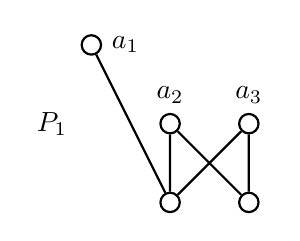
\begin{tikzpicture}[lattice/.style={thick,circle,draw=black,fill=white,inner sep=0pt, minimum size=7pt}]
            \node[lattice] (a) at (0,0) {};
            \node[lattice,label=above:{$a_2$}] (c) at  (0,1) {};
            \node[lattice,label=above:{$a_3$}] (d) at  (1,1) {};
            \node[lattice] (b) at  (1,0) {};
            \node[lattice,label=right:{$a_1$}] (e) at (-1,2) {};
            
            \draw[thick] (e)--(a)--(c)--(b)--(d)--(a);
            \node at (-1.5,1) {$P_1$};
        \end{tikzpicture}    
    \end{minipage}
    \begin{minipage}[b]{0.4\textwidth}
        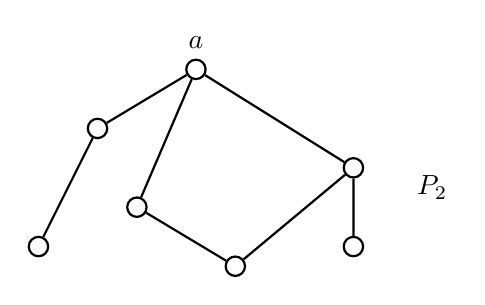
\begin{tikzpicture}[lattice/.style={thick,circle,draw=black,fill=white,inner sep=0pt, minimum size=7pt}]
            \node[lattice] (aa) at (0,0) {};
            
            \node[lattice] (a) at  (-2.5, 0.25) {};
            \node[lattice] (b) at  (1.5, 0.25) {};
            \node[lattice] (c) at  (-1.25,.75) {};
            \node[lattice] (d) at (1.5,1.25) {};
            \node[lattice] (e) at (-1.75,1.75) {};
            \node[lattice,label=above:{$a$}] (f) at (-0.5,2.5) {};
            
            \draw[thick] (b)--(d)--(aa)--(c)--(f)--(e)--(a) (f)--(d);
            \node at (2.5,1) {$P_2$};
        \end{tikzpicture}
    \end{minipage}
\end{figure}
In the above figure \(P_1\) has maximal elements \(a_1\), \(a_2\), \(a_3\), but no greatest element; \(a\) is the greatest element of \(P_2\).


Let \(P\) be a finite ordered set. Then any non-empty subset of \(P\) has at least one maximal element and, for each \(x\in P\), there exists \(y\in \max P\) with \(x\leq y\). In general a subset \(Q\) of an ordered set \(P\) may have many maximal elements, just one, or none. A subset of the chain \(\N\) has a maximal element if and only if it is finite and non-empty.
\section{Sums of Ordered Sets}
\subsection{Disjoint Union}
Suppose that \(P\) and \(Q\) are (disjoint) ordered sets. The disjoint union \(P\,
\dot{\cup}\, Q\) of \(P\) and \(Q\) is the ordered set formed by defining \(x \leq y\) in \(P\,\dot{\cup}\, Q\) if and only if either \(x,\, y \in P\) and \(x \leq y\) in \(P\) or \(x,\, y \in Q\) and \(x \leq y\) in \(Q\). A diagram for \(P\,\dot{\cup}\, Q\) is formed by placing side by side diagrams for \(P\) and \(Q\).
\subsection{Linear Sum}
Let \(P\) and \(Q\) be (disjoint) ordered sets. The linear sum \(P \oplus Q\) is defined by taking the following order relation on \(P\,\cup\,Q:\;x \leq y\) if and only if
\begin{align*}
    &x,\,y \in P \text{ and } x \leq y \text{ in } P,\\
    \text{or}\quad& x,\,y \in Q \text{ and } x \leq y \text{ in } Q,\\
    \text{or}\quad& x \in P \text{ and } y\in  Q.
\end{align*}
A diagram for \(P \oplus Q\) (when \(P\) and \(Q\) are finite) is obtained by placing a diagram for \(P\) directly below a diagram for \(Q\) and then adding a line segment from each maximal element of \(P\) to each minimal element of \(Q\).
\begin{note}
    Each of the operations \(\dot{\cup}\) and \(\oplus\) is associative; for (pairwise disjoint) ordered sets \(P\), \(Q\) and \(R\),
    \[
        P\,\dot{\cup}\,(Q\,\dot{\cup}\,R) = (P\,\dot{\cup}\,Q)\,\dot{\cup}\,R \qquad\text{and}\qquad P \oplus (Q \oplus R) = (P \oplus Q) \oplus R
        \]
\end{note}
\subsection{Examples}
\begin{enumerate}
    \item\hfill
    \begin{figure}[H]
        \centering
        \import{../tikz/}{twoThree.tikz}
        \caption{\(P=\mathbf{2}\), \(Q=\mathbf{3}\), \(P\;\dot\cup\; Q=\mathbf{2}\;\dot\cup\;\mathbf{3}\) and \(P\oplus Q=\mathbf{2}\oplus\mathbf{3}\cong \mathbf{5}\)}
    \end{figure}
    \item \hfill
    \begin{figure}[H]
        \centering
        \import{../tikz/}{m3m2.tikz}
        \caption{\(P=M_3\), \(Q=M_2\), \(P\;\dot\cup\; Q=M_3\;\dot\cup\;M_2\) and \(P\oplus Q=M_3\oplus M_2\)}
    \end{figure}
    \item For \(P\oplus Q\), we consider \(P=\bar{\mathbf{1}}\), \(Q=\bar{\mathbf{2}}\), \(R=\bar{\mathbf{3}}\).\\
    % \begin{center}
        \begin{tikzpicture}
            \node at (0,1) {};
            \node  at (-1.5,0) {\(\therefore P\oplus Q=\)};
            \node[lattice] at (0,0) {};
            \node[lattice] at (1.75,0) {};
            \node[lattice] at (2.25,0) {};
            \node  at (1,0) {$\oplus$};
            \node  at (3,0) {$\cong$};
            \node[lattice] (a) at (5,-.5) {};
            \node[lattice] (b) at (4,.5) {};
            \node[lattice] (c) at (6,.5) {};
            \draw[thick] (b)--(a)--(c);
        \end{tikzpicture}\\
    % \end{center}
    \begin{tikzpicture}
        \node  at (-3,0) {Also, \(P\oplus Q \oplus R=\)};
        
        \node[lattice] at (2.5,0) {};
            \node[lattice] at (3,0) {};
            \node[lattice] at (3.5,0) {};
            \node  at (1.5,0) {$\oplus$};
            \node  at (4.5,0) {$\cong$};
            \node[lattice] (a) at (0,-.5) {};
            \node[lattice] (b) at (-1,.5) {};
            \node[lattice] (c) at (1,.5) {};
        \draw[thick] (b)--(a)--(c);
        
        \node[lattice] (A) at (5,1.5) {};
            \node[lattice] (B) at (7,1.5) {};
            \node[lattice] (C) at (9,1.5) {};
        \node[lattice] (aa) at (7,-.5) {};
            \node[lattice] (ba) at (6,.5) {};
            \node[lattice] (ca) at (8,.5) {};
        \draw[thick] (ba)--(aa)--(ca);
        \draw[thick] (A)--(ba)--(B);
        \draw[thick] (B)--(ca)--(C);
        \draw[thick] (A)--(ca) (ba)--(C);
        \end{tikzpicture}
    \item \begin{tikzpicture}
        \node  at (-3,0) {\(1\oplus 2^2=\)};
        
        \node[lattice] at (-2,0) {};
        \node  at (-1,0) {$\oplus$};
        \node[lattice] (0) at (1,-1) {};
        \node[lattice] (a) at (0,0) {};
        \node[lattice] (b) at (2,0) {};
        \node[lattice] (1) at (1,1) {};
        \draw[thick] (0)--(a)--(1)--(b)--(0);
        \node  at (3,0) {$\cong$};
        \node[lattice] (000)at (5,-2) {};
        \node[lattice] (00) at (5,-1) {};
        \node[lattice] (0a) at (4,0) {};
        \node[lattice] (0b) at (6,0) {};
        \node[lattice] (01) at (5,1) {};
        \draw[thick] (00)--(0a)--(01)--(0b)--(00)--(000);
    \end{tikzpicture}\\
    
    \begin{tikzpicture}
\node  at (8,0) { and };
\node  at (10,0) {\(2^2\oplus 1=\)};
        \node[lattice] at (15,0) {};
            \node  at (14,0) {$\oplus$};
            \node[lattice] (10) at (12,-1) {};
            \node[lattice] (1a) at (11,0) {};
            \node[lattice] (1b) at (13,0) {};
            \node[lattice] (11) at (12,1) {};
        \draw[thick] (10)--(1a)--(11)--(1b)--(10);
        \node  at (14,0) {$\cong$};
        \node[lattice] (1000)at (17,2) {};
            \node[lattice] (100) at (17,-1) {};
            \node[lattice] (10a) at (16,0) {};
            \node[lattice] (10b) at (18,0) {};
            \node[lattice] (101) at (17,1) {};
        \draw[thick] (1000)--(101) (100)--(10a)--(101)--(10b)--(100);
        \end{tikzpicture}
    \item a
\end{enumerate}
\end{document}